\section{Message Passing Algorithms on Trees}

If the factor graph is a tree, many problems can be solved efficiently using a form of dynamic programming called \emph{message passing}. \newline 
In general, message passing algorithms compute values for each edge of the factor graph. These values can be interpreted as \emph{messages} that are sent between the nodes. Since all edges connect factor nodes to variable nodes there can be two types of messages: messages passed from a variable $i$ to a factor $a$, denoted as $m_{i \rightarrow a}$ and messages passed from $a$ to $i$, denoted as $m_{a \rightarrow i}$. \newline
The messages must be defined so that a message $m_{a \rightarrow i}$ is determined by the messages $m_{j \rightarrow a}$ that $a$ received from neighbour variables $j \neq i$. 
The same must hold for $m_{i \rightarrow a}$. \newline
Usually the massages $m_{i \rightarrow a}$ are obtained by summing over $m_{b \rightarrow i}$ and $m_{a \rightarrow i}$ by multiplying the messages $m_{j \rightarrow a}$. The fundamental equation usually has the form $m_{i \rightarrow a} = \sum_{j \in V(a) \setminus i} \prod_{b \in V(j) \setminus a} m_{j \rightarrow b}$. Therefore these types of algorithms are called \emph{sum-product}-algorithms. \newline
For tree factor graphs which do not contain cycles the value of $m_{i \rightarrow a}$ does not influence its predecessors $m_{b \rightarrow i}$. The messages can be computed sequentially starting with the factor graphs's leaves.


\section{Message Passing on general graphs}
If a graph contains cycles, the above described messages are in general not well-defined. However, message passing algorithms which are correct for trees can be used as a heuristic for general graphs. \newline
This \emph{loopy} form of message passing consists of two parts. In the initialization  step each message is provisionally assigned a random value. Now that each message is set the sum-product equation can be used not to compute the absolute result but to update the provisional values. The update steps are repeatedly performed for each edge $i \rightarrow a$ in random order. The goal is to reach a point where no message would significantly change when applying the update rule to it. If this is the case, the messages are said to have \emph{converged}. Since there is no guarantee for convergence it is also possible for the update process to never terminate. In this case the computation has to be terminated after a fixed number of steps. \newline
In practice the update rule has to be slightly modify when applying message passing on loopy graphs. Since the messages are computed from random starting values they often do not fulfill properties which the original defined messages do.

On trees this heuristical approach still returns correct results, on general graphs experience shows that convergence happens rather frequently.

\begin{lemma}
Loopy message passing converges on trees.
\end{lemma}

\begin{itemize}
	\item "Loopy" belief propagation
	\item Convergence for trees
	\item Heuristic for general graphs
	\item Examples only in next chapter
\end{itemize}

\begin{figure}[h]
\centering

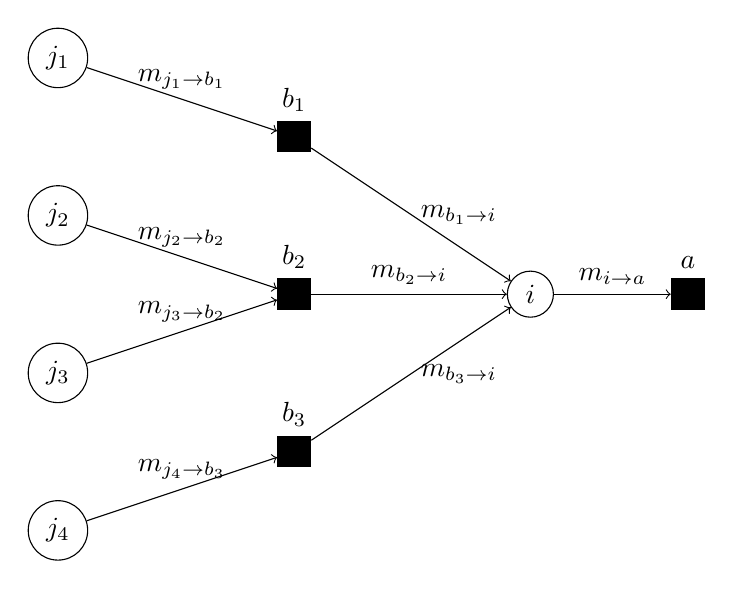
\begin{tikzpicture}[scale=1.0,transform shape]
   	\node[rectangle,draw=black, label = {$a$}, fill] (a) at (5,0) {$a$};
    \node[shape=circle,draw=black] (i) at (3,0) {$i$};
   
  \node[rectangle,draw=black, label = {$b_1$}, fill] (b1) at (0,2) {$a$};
  \node[rectangle,draw=black, label = {$b_2$}, fill] (b2) at (0,0) {$a$};
  \node[rectangle,draw=black, label = {$b_3$}, fill] (b3) at (0,-2) {$a$};

	\node[shape=circle,draw=black] (j1) at (-3,3) {$j_1$};
	\node[shape=circle,draw=black] (j2) at (-3,1) {$j_2$};
	\node[shape=circle,draw=black] (j3) at (-3,-1) {$j_3$};
	\node[shape=circle,draw=black] (j4) at (-3,-3) {$j_4$};


    
	\draw[->] (b3) edge [right] node {$m_{b_3 \rightarrow i}$} (i);
	\draw[->] (b2) edge [above] node {$m_{b_2 \rightarrow i}$} (i);
	\draw[->] (b1) edge [right] node {$m_{b_1 \rightarrow i}$} (i);
	\draw[->] (i) edge [above] node {$m_{i \rightarrow a}$} (a);
	
	\draw[->] (j1) edge [above] node {$m_{j_1 \rightarrow b_1}$} (b1);
  	\draw[->] (j2) edge [above] node {$m_{j_2 \rightarrow b_2}$} (b2);
	\draw[->] (j3) edge [above] node {$m_{j_3 \rightarrow b_2}$} (b2);
	\draw[->] (j4) edge [above] node {$m_{j_4 \rightarrow b_3}$} (b3);

\end{tikzpicture}
\caption{Factor graph of a SAT formula}
\end{figure}